\documentclass{article}
\PassOptionsToPackage{numbers,sort&compress}{natbib}
\ifdefined\AnonymousSubmission
  \usepackage{neurips_2024}
\else
  \usepackage[preprint]{neurips_2024}
\fi
\usepackage[utf8]{inputenc}
\usepackage[T1]{fontenc}
\usepackage{amsmath,amsfonts,booktabs,graphicx,microtype,url,hyperref,xcolor}
\hypersetup{hidelinks}
% Preserve the supplied layout. Correct only its misleading submission-status notice.
\makeatletter
\renewcommand{\@noticestring}{Research draft. Not submitted to a conference.}
\makeatother
\title{Auditing Audio--Lyrics Variational Autoencoders\\for Music Clustering}
\author{Sm Azmain Faysal\\Department of Computer Science\\BRAC University\\
\texttt{sm.azmain.faysal@g.bracu.ac.bd}}
\newcommand{\NTrain}{478}
\newcommand{\NVal}{103}
\newcommand{\NTest}{102}

\begin{document}
\maketitle
\begin{abstract}
Variational autoencoders (VAEs) can produce compact music representations, but a
high internal clustering score does not establish agreement with musical genres.
We audit a course project containing spectrograms and lyrics for 683 songs and
rebuild its evaluation with ID alignment, train-only preprocessing, grouped
held-out splits, and five random seeds. The archived beta-VAE and conditional
VAE produce silhouette scores of 0.894 and 0.954 while assigning more than 99\%
of songs to one cluster; their adjusted Rand indices (ARI) are approximately
zero. The rebuilt study compares audio, text, and multimodal representations,
regularization strengths, and negative controls using a fixed test set of
\NTest{} songs. The convolutional audio--lyrics hybrid reaches ARI $0.207\pm0.029$, compared with $0.096\pm0.020$ for an audio VAE and $0.227\pm0.028$ for text-only features. The results support a benefit over audio alone, but do not establish an advantage over text alone.

Two additional grouped splits preserve this ordering.

We report uncertainty, reconstruction quality, latent diagnostics and the
limitations of the supplied data. A separate English--Bangla experiment addresses
the course's bilingual requirement; it is a feasibility study, not evidence of
language-invariant genre discovery. The contribution is a reproducible empirical
audit and corrected benchmark, rather than a claim of a new VAE architecture.
\end{abstract}

\section{Introduction}
Music clustering can support the exploration of collections without training a
genre classifier. Audio and lyrics offer different information: acoustic
representations describe recorded sound, while lyric representations can reflect
vocabulary and subject matter. Their combination is a plausible representation
learning strategy, but reconstruction quality, cluster geometry and semantic
agreement are distinct objectives. A low-dimensional embedding can be easy to
partition without recovering the categories that matter to a listener.

The original course project explored dense, convolutional, multimodal and
conditional VAEs. Its archive contains inconsistent data descriptions,
preprocessing fitted before splitting, decoder outputs incompatible with some
target values, and conclusions that do not follow from the reported metrics.
This study repairs those issues and asks three concrete questions: (1) do stronger
internal scores correspond to genre agreement; (2) does joint audio--lyrics
learning improve on unimodal and linear baselines; and (3) how do KL weighting
and modality pairing affect the learned representation?

We provide an executable benchmark with preserved legacy evidence, source hashes,
saved splits, fitted transformations and checkpoints. We distinguish fully
unsupervised training from a genre-conditioned oracle, and distinguish inductive
clustering from within-test descriptive clustering. We also evaluate a small
bilingual cohort independently, because the supplied arrays do not establish the
English--Bangla coverage required by the assignment. These are empirical and
reproducibility contributions; we do not claim a novel algorithm or demonstrated
disentanglement.

\section{Related work}
VAEs learn a probabilistic latent representation using an approximate posterior
and a reparameterized training objective \citep{kingma2014vae}. A beta-VAE changes
the relative strength of prior regularization \citep{higgins2017betavae}, while
free-bits objectives avoid penalizing small per-component KL values
\citep{kingma2016iaf}. Posterior collapse concerns the relationship between the
posterior and prior, not just an imbalanced clustering result
\citep{he2019lagging}. Moreover, unsupervised disentanglement cannot generally be
identified without assumptions about models and data \citep{locatello2019}.
Accordingly, we measure KL, active units and effective rank, and do not infer
disentanglement from a visualization.

Multimodal VAEs have been developed with explicit mechanisms for combining
modalities and handling missing observations \citep{wu2018mvae}. Our
concatenation-based models are simpler and require both inputs; they do not
implement product-of-experts inference. Research on lyric topics and genre
\citep{aljanaki2024} motivates testing a text-only baseline before crediting
joint learning. We use PCA and deterministic autoencoders as audio controls,
and TF-IDF with truncated SVD as an auditable text representation. t-SNE
\citep{vandermaaten2008tsne} is used only for visualization. Two-dimensional
separation is not an evaluation criterion.

\section{Data and audit}
\label{sec:data}
The supplied metadata has 796 rows with track ID, title, audio path, genre and
lyrics. Saved processed IDs identify 683 unique rows, each paired with a
$128\times256$ array. The genre counts are rock 178, rap 178, pop 153, country
109 and rb 65. Metadata is joined in the exact processed-ID order. A membership
filter happens to preserve this archive's order, but is not an adequate general
alignment procedure. Another notebook failed by comparing 683 representations
with 796 labels; a separate 500-example synthetic notebook is excluded.

The stored arrays are finite and range from $-1$ to $1$. None of the referenced
raw audio files is present. Thus we can reproduce experiments from the supplied
features, but cannot independently establish the original sample rate,
spectrogram construction, clipping, or normalization. The accompanying source attribution points to a
GTZAN Kaggle mirror, and the processed files were received from a collaborator. This does not establish an ID-level mapping
to that benchmark. We therefore call this the \emph{supplied corpus}, not a
verified GTZAN subset.

The archive also contains a $683\times384$ lyric embedding matrix without a
model revision or row-ID sidecar. Its dimensions do not identify it as BERT.
We do not use it in the new primary experiments. Instead, text features are
computed from the aligned lyrics. There is no language column and no
Bengali-script text in the processed lyrics. Script absence is not a language
annotation; multilingual results cannot be inferred from this corpus.

\paragraph{Legacy evidence.}
Reclustering the saved means reproduces the main pathological scores
(Table~\ref{tab:legacy}). The beta-VAE K-means partition has sizes
$[679,1,1,1,1]$ and the conditional model has $[678,1,1,1,2]$. Both have zero
active units at the variance threshold used below. Saved posterior variances
are unavailable, so this establishes low dispersion and degenerate partitions,
not a complete posterior-collapse diagnosis. The old ``Spectral'' baseline was
a second PCA of the same input; it was not an independent spectral baseline.
\begin{table}[htbp]
\centering
\caption{Recomputed legacy K-means results on all 683 saved embeddings, seed 42. These are in-sample diagnostics, not comparable held-out scores.}
\label{tab:legacy}
\small
\begin{tabular}{lrrr}
\toprule
Saved representation & Silhouette & ARI & Largest share \\
\midrule
Conv VAE & 0.295 & 0.044 & 0.378 \\
Dense VAE & 0.202 & 0.034 & 0.268 \\
Beta-VAE & 0.894 & -0.001 & 0.994 \\
Conditional VAE & 0.954 & 0.000 & 0.993 \\
PCA & 0.103 & 0.067 & 0.322 \\
\bottomrule
\end{tabular}
\end{table}


\section{Method}
\label{sec:method}
\subsection{Preprocessing and representations}
A fixed $4\times4$ average pool reduces each supplied spectrogram to
$32\times64$. The pooled values are centered and scaled using a single mean
and standard deviation from training data. This makes local CPU experiments
tractable and is an explicit change from the original full-resolution models.
No physical frequency or time calibration is inferred for the cached arrays.

For lyrics, literal newline escapes are replaced by spaces. A word unigram and
bigram TF-IDF vocabulary is learned on training songs only, with sublinear term
frequency, minimum document frequency 2, maximum document frequency 0.95, and at
most 10,000 terms. Truncated SVD produces 64 features, standardized using the
training set. The text-only comparator projects these to 32 dimensions with
PCA. The procedure is reproducible and does not require guessing a pretrained
transformer identity.

All primary learned embeddings have dimension $d_z=32$. The dense audio encoder
has widths $2048\rightarrow256\rightarrow128$, followed by a 128-unit fusion
layer and separate mean and log-variance heads. The decoder uses
$32\rightarrow128\rightarrow256\rightarrow2048$. Hidden layers use ReLU;
output layers are linear because targets are signed continuous features.
The convolutional encoder uses three stride-2, $3\times3$ layers with 8, 16 and
32 channels, producing a $32\times4\times8$ map, followed by 128 units. Its
decoder uses a dense projection and three stride-2 transposed convolutions with
$4\times4$ kernels. The dense multimodal model adds a
$64\rightarrow128\rightarrow64$ text encoder and concatenates the audio and
text branches before the fusion layer. The hybrid replaces the dense audio
branch by the convolutional branch. A $32\rightarrow128\rightarrow64$ decoder
reconstructs text in both multimodal models.

\subsection{Objective and regularization}
The encoder defines a diagonal Gaussian posterior
$q_\phi(z\mid x)=\mathcal N(\mu,\operatorname{diag}(\exp\ell))$.
Sampling uses $z=\mu+\exp(\ell/2)\odot\epsilon$, where
$\epsilon\sim\mathcal N(0,I)$. We clamp $\ell$ to $[-12,12]$ for numerical
stability. Let $D_a=2048$ and $D_t=64$. The implemented objective is
\begin{equation}
\label{eq:loss}
\mathcal J =
 \mathbb E_{q}\!\left[\frac{\lVert x_a-\hat x_a\rVert_2^2}{D_a}
 +\mathbf1_{\rm multimodal}\frac{\lVert x_t-\hat x_t\rVert_2^2}{D_t}\right]
 +\frac{\beta}{d_z}\sum_{j=1}^{d_z}\bar K_j,
\qquad
K_j=\tfrac12(\mu_j^2+e^{\ell_j}-1-\ell_j),
\end{equation}
where $\bar K_j$ is the minibatch mean KL for dimension $j$.
This is a dimension-normalized, weighted reconstruction--KL objective, not a
reported likelihood bound with a calibrated observation variance. Its beta
values are not directly comparable to those of a sum-reconstruction ELBO.
Audio-only beta values are $0.001,0.01,0.1,1$. The multimodal, convolutional and
hybrid models use $0.01$. A free-bits ablation replaces
$\bar K_j$ by $\max(\bar K_j,0.05)$. The autoencoder decodes $\mu$ directly with
no sampling or KL penalty.

\paragraph{Controls.}
PCA retains 32 dimensions of flattened pooled audio. A second baseline uses
per-frequency temporal mean and standard deviation, standardized and reduced
to 32 dimensions. Direct spectral clustering uses all 2,048 pooled values
without PCA. Fusion PCA concatenates audio and text after separately scaling
each modality to unit total training variance, then retains 32 components.
A negative control independently permutes lyrics within each split before
training and evaluation. It preserves text marginals while destroying track
pairing. Genre-conditioned audio and multimodal VAEs concatenate a genre
one-hot vector at the encoder and audio decoder. They require known genre at
test time, so their results are labeled \emph{oracle}, outside the unsupervised
comparison.

\subsection{Clustering and diagnostics}
K-means uses 20 initializations, fits training means, and predicts validation
and test assignments. Five clusters are fixed from the course setting and
known category count; genre labels otherwise do not enter unsupervised training
or model selection. We also report $k\in\{2,3,4,6,8,10\}$ without selecting a
winner on test labels. Embeddings are centered and divided by one global
training RMS norm, which preserves Euclidean relative geometry. We do not
whiten each latent dimension and amplify near-constant coordinates.

Ward agglomeration and DBSCAN are fitted directly to test embeddings and are
reported as separate \emph{transductive} descriptions, not out-of-sample
predictors. DBSCAN uses five neighbors. Radius candidates are the training
fifth-neighbor median and 90th percentile times $0.5,1,2$, selected by validation
coverage times silhouette minus noise fraction; invalid partitions score $-2$.
Noise is excluded from partition metrics and its fraction is always reported.
One-cluster, all-noise or singleton-only partitions have undefined internal
scores, retained as missing values.

We compute silhouette, Davies--Bouldin, Calinski--Harabasz, ARI, arithmetic NMI,
adjusted mutual information, and purity. A majority-class purity baseline,
largest-cluster fraction and effective cluster count contextualize the results.
Active units satisfy $\operatorname{Var}(\mu_j)>0.01$. Effective rank is the
exponential entropy of the normalized squared singular values of centered
means. Internal scores are geometry-specific; their magnitudes across different
representations are not calibrated measures of semantic usefulness.

\section{Experiments}
\label{sec:experiments}
Duplicate groups join equal normalized titles, normalized lyrics, or exact
spectrogram arrays. This yields 676 groups and a fixed group-disjoint split
(seed 2026) of \NTrain{} training, \NVal{} validation and \NTest{} test songs.
Genre is not used to stratify the split. Artist identifiers are unavailable;
artist or recording-family independence cannot be claimed. All transformations,
including vocabulary, SVD, scalers and PCA, fit only training rows.

We use CPU PyTorch on an Apple M1 MacBook Air (8 GB RAM), four computation threads, Adam with learning rate $10^{-3}$,
batch size 64, gradient norm clipping at 5, and at most 100 epochs. KL weight
increases linearly over 20 epochs. Checkpoint selection starts at epoch 20 and
minimizes the full-weight validation objective, with patience 15. Validation
uses four fixed Gaussian samples per song, shared across epochs for a model.
Training seeds are 11, 22, 33, 44 and 55. We report sample standard deviations
across runs on the same split; these do not measure between-dataset uncertainty.
The 60 trained neural-model runs in the primary study and requirement extension took 6.4 minutes of summed local training wall time, excluding environment setup, clustering, reporting and the separate bilingual study. Selected epochs ranged from 25 to 100; parameter counts ranged from 206,041 to 1,184,320.

The additional split-sensitivity study trained 60 neural models in 7.9 minutes of summed training wall time; preprocessing and evaluation are additional.


\paragraph{Bilingual course experiment.}
We obtain 20 explicitly English-labeled recordings from JamendoLyrics \citep{durand2023} and 20 Bengali clips from BanglaBeats \citep{jibon2023}. Repository revisions and file hashes are pinned. English excerpts start at the first annotated sung line and last three seconds; Bengali excerpts are the released three-second clips, selected at spaced numeric file ranks across eight genres. A shared new recipe uses mono 22,050-Hz audio, FFT size 2,048, hop 512, 128 mel bins, per-clip relative dB clipped at $-80$ dB, and linear time interpolation to 256 frames, followed by the same pooling. A fixed language-stratified split uses 32 clips for fitting and eight for validation, with an eight-dimensional VAE and PCA. This separate course demonstration fits and evaluates K-means on all 40 representations; it is explicitly transductive and makes no held-out performance claim. BanglaBeats does not provide original song IDs in this release, so distinct-song independence cannot be verified. It also provides no matched lyrics; the multimodal study remains on the supplied corpus.


\section{Results}
\label{sec:results}
\subsection{Held-out genre agreement}
\begin{table}[htbp]
\centering
\caption{Inductive K-means on held-out songs, $k=5$. Mean $\pm$ sample SD over five seeds; higher is better for the displayed metrics.}
\label{tab:main}
\small
\begin{tabular}{lrrrr}
\toprule
Representation & ARI & NMI & Silhouette & Purity \\
\midrule
Direct spectral & $0.086\pm0.000$ & $0.128\pm0.000$ & $0.157\pm0.000$ & $0.441\pm0.000$ \\
Audio PCA & $0.086\pm0.000$ & $0.128\pm0.000$ & $0.236\pm0.000$ & $0.441\pm0.000$ \\
Audio statistics & $0.084\pm0.003$ & $0.121\pm0.008$ & $0.264\pm0.003$ & $0.449\pm0.004$ \\
Lyrics LSA & $0.227\pm0.028$ & $0.258\pm0.017$ & $0.056\pm0.012$ & $0.541\pm0.013$ \\
Fusion PCA & $0.089\pm0.010$ & $0.119\pm0.005$ & $0.236\pm0.006$ & $0.447\pm0.005$ \\
Audio AE & $0.072\pm0.010$ & $0.119\pm0.023$ & $0.292\pm0.024$ & $0.422\pm0.030$ \\
Audio VAE (0.01) & $0.096\pm0.020$ & $0.128\pm0.017$ & $0.218\pm0.016$ & $0.449\pm0.021$ \\
Conv VAE & $0.068\pm0.007$ & $0.103\pm0.016$ & $0.226\pm0.030$ & $0.418\pm0.021$ \\
Multimodal VAE & $0.153\pm0.096$ & $0.177\pm0.094$ & $0.195\pm0.038$ & $0.467\pm0.064$ \\
Hybrid VAE & $0.207\pm0.029$ & $0.241\pm0.037$ & $0.149\pm0.041$ & $0.516\pm0.019$ \\
\bottomrule
\end{tabular}
\end{table}

Table~\ref{tab:main} shows a hybrid ARI of $0.207\pm0.029$ against $0.096\pm0.020$ for the audio VAE at $\beta=0.01$ and $0.086\pm0.000$ for audio PCA. The paired hybrid-minus-audio-VAE difference is 0.111, with an exploratory 95\% bootstrap interval [0.030, 0.195]. Text-only LSA obtains $0.227\pm0.028$ ARI. The hybrid-minus-text difference is -0.020, interval [-0.126, 0.092], so these data do not establish a hybrid advantage over text. Test-set majority-class purity is 0.304. The comparison concerns a fixed corpus and split, not general superiority of one architecture.

\paragraph{Split sensitivity.}
Two follow-up group-disjoint splits (seeds 2027 and 2028) repeat six neural models and four baselines with the same five training seeds and unchanged hyperparameters (Table~\ref{tab:robustness}). The hybrid-minus-audio-VAE mean ARI differences across splits 2026, 2027 and 2028 are +0.111, +0.090, +0.140; hybrid-minus-text differences are -0.020, -0.085, -0.089. These follow-up evaluations assess split sensitivity after inspecting the primary results; they are not independent dataset replications or confirmatory tests.

\begin{figure}[t]
\centering
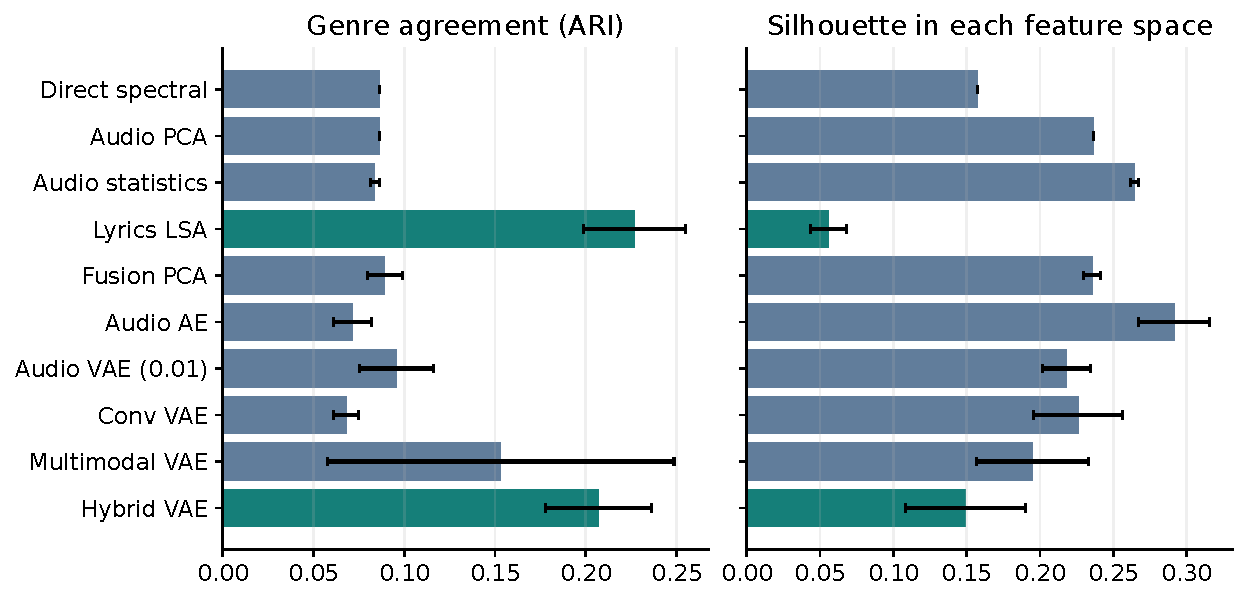
\includegraphics[width=\linewidth]{figures/rebuilt_performance.pdf}
\caption{Held-out genre agreement (ARI) and within-representation silhouette.
Bars show means over five seeds; error bars show sample standard deviation.
Semantic and geometric rankings need not agree. Oracle models are excluded.}
\label{fig:performance}
\end{figure}

\subsection{Regularization and modality controls}
\begin{table}[htbp]
\centering
\caption{Regularization and pairing controls on the same held-out split. FB denotes a 0.05-nat free-bits threshold per latent dimension.}
\label{tab:ablation}
\small
\begin{tabular}{lrrr}
\toprule
Representation & ARI & Silhouette & Largest share \\
\midrule
Audio VAE (0.001) & $0.070\pm0.010$ & $0.247\pm0.009$ & $0.376\pm0.026$ \\
Audio VAE (0.01) & $0.096\pm0.020$ & $0.218\pm0.016$ & $0.329\pm0.016$ \\
Audio VAE (0.1) & $0.067\pm0.018$ & $0.251\pm0.016$ & $0.373\pm0.048$ \\
Audio VAE (1) & $0.067\pm0.012$ & $0.435\pm0.023$ & $0.363\pm0.018$ \\
Multimodal VAE & $0.153\pm0.096$ & $0.195\pm0.038$ & $0.406\pm0.064$ \\
Multimodal + FB & $0.172\pm0.078$ & $0.197\pm0.055$ & $0.402\pm0.044$ \\
Shuffled text & $0.032\pm0.012$ & $0.149\pm0.024$ & $0.480\pm0.105$ \\
\bottomrule
\end{tabular}
\end{table}

The dense multimodal model obtains ARI $0.153\pm0.096$, whereas shuffled pairing obtains $0.032\pm0.012$. The negative control indicates that preserving the relation between a song and its lyrics matters in this setup. Free bits gives $0.172\pm0.078$, but the large run variation prevents a robust superiority claim. Raising audio $\beta$ to 1 increases mean silhouette to 0.435 while ARI remains 0.067. Figure~\ref{fig:beta} reports the associated latent and reconstruction changes; a higher geometry score alone is not evidence of improvement.

\begin{figure}[t]
\centering
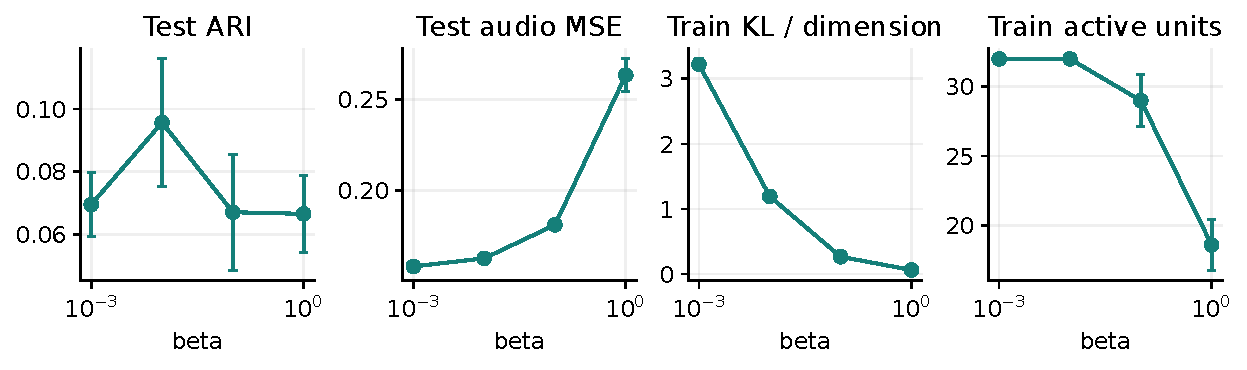
\includegraphics[width=\linewidth]{figures/rebuilt_beta.pdf}
\caption{Audio VAE regularization sweep: test genre agreement, test reconstruction
MSE at the posterior mean, training KL per dimension and training active units.
All panels use five-seed means with sample standard deviations.}
\label{fig:beta}
\end{figure}

\subsection{Reconstructions and latent visualization}
\begin{figure}[t]
\centering
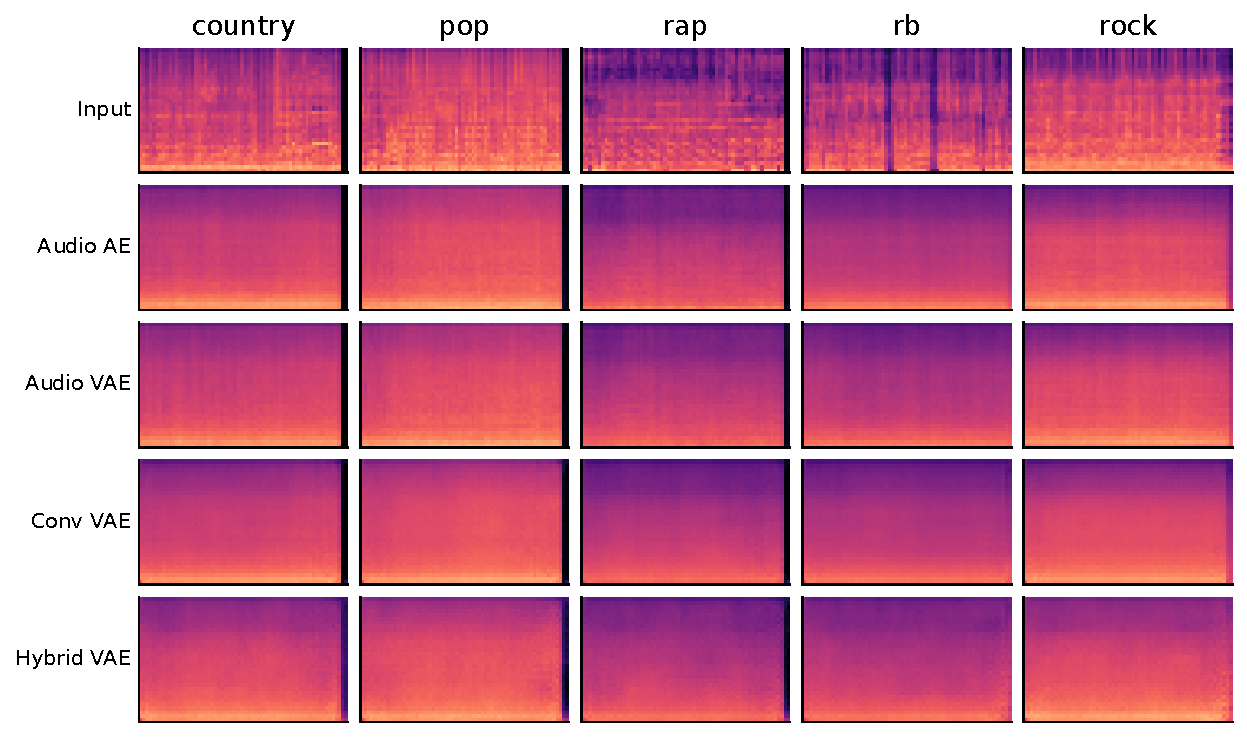
\includegraphics[width=\linewidth]{figures/rebuilt_reconstruction.pdf}
\caption{Pooled inputs and posterior-mean reconstructions for the first test
example in each genre, using seed 11. Every panel uses the same normalized
value range of $[-3,3]$. Reconstructed coarse structure does not demonstrate perceptual
audio quality or genre disentanglement.}
\label{fig:reconstruction}
\end{figure}
The reconstructed arrays show how models allocate capacity to the cached
features (Figure~\ref{fig:reconstruction}). The raw waveforms are unavailable;
we do not claim waveform reconstruction or perceptual quality. Appendix plots
show test t-SNE projections, genre contingency tables, cluster sizes,
interpolation and $k$ sensitivity. A t-SNE fit is descriptive and is never used
to compute the reported clustering metrics.

\subsection{Bilingual feasibility results}
\begin{table}[htbp]
\centering
\caption{Small bilingual demonstration, $k=5$, mean $\pm$ SD. K-means fits and scores all 40 clips, including training clips. ARI compares language, which equals source.}
\label{tab:bilingual}
\small
\begin{tabular}{lrrr}
\toprule
Representation & Silhouette & CH & Language ARI \\
\midrule
PCA & $0.175\pm0.026$ & $10.025\pm0.222$ & $0.003\pm0.010$ \\
VAE & $0.376\pm0.023$ & $54.907\pm5.140$ & $-0.005\pm0.011$ \\
\bottomrule
\end{tabular}
\end{table}

Both languages pass through a common audio preprocessing and clustering implementation. Table~\ref{tab:bilingual} reports internal scores and language agreement for all clips. Language is perfectly confounded with dataset source and may also covary with genre, recording practice and excerpt selection. These numbers therefore demonstrate execution on bilingual inputs; they do not establish language recognition, language-invariant music structure or generalization to new songs. The appendix plots actual language counts in each cluster.


\section{Discussion and limitations}
\label{sec:limitations}
The original ``VAE always outperforms PCA'' conclusion is not supported. High
silhouette can coexist with near-chance genre agreement, and reconstructing
both modalities does not automatically make their joint representation more
useful than text alone. Genre is also only one imperfect description of music;
low ARI does not exclude grouping by another meaningful attribute, but evidence
for such attributes requires annotations or a listening study.

The main corpus is small and provenance is incomplete. The primary test set
contains only six rb examples. Two additional grouped splits assess sensitivity,
but all three reuse the same corpus. Five optimization seeds
and conditional bootstrap intervals cannot substitute for independent datasets
or artist-disjoint evaluation. The vocabulary/SVD representation is an
interpretable baseline rather than a modern pretrained music or multilingual
language model. Fixed pooling discards resolution. Cross-model reconstruction
objectives differ when text is added, so total losses are not used to rank
unimodal against multimodal models. The bilingual cohort is small and its
language labels are confounded with collection source. It addresses an
implementation requirement, not a causal claim about language.

Data licenses and original extraction provenance for the supplied corpus remain
unresolved. The local package contains research artifacts, but is not evidence
of permission to redistribute songs or lyrics. Public release should provide
source-specific access instructions and verified licensing. Model weights and
reconstructions can retain information about the training material. Broader
applications would also require evaluation of language and genre coverage to
avoid presenting an uneven collection as culturally representative.

A conference submission requires a clearer generalizable finding, replication
on documented datasets, suitable pretrained audio/text baselines, and review of
any target venue's current format and policies. The present repaired benchmark
is a basis for that work, not a claim that a top-tier submission is ready.

\section{Conclusion}
This study repairs a music VAE project by connecting every reported result to
an executable, ID-aligned evaluation. It replaces unsupported multilingual and
transformer claims with explicit data provenance, separates genre-conditioned
oracles from unsupervised models, and demonstrates why cluster geometry must
be interpreted alongside semantic agreement and balance. The measured
comparisons establish a reproducible baseline for subsequent research;
stronger generalization and language-invariance claims require further data.

\clearpage
\bibliographystyle{plainnat}
\bibliography{references}

\section*{AI assistance and author review}
An AI coding assistant was used to audit the supplied files, implement and run
experiments, generate figures, check references, and revise this manuscript.
The named author must independently review the code, results, dataset rights
and scientific claims before submission. No human listening study, new
annotation study, or independent author verification is claimed here.

\clearpage
\appendix
\section{Reproduction and full results}
\label{app:repro}
The repository README provides environment setup and exact commands.
\texttt{configs/main.json} specifies the frozen primary study.
\texttt{results/rebuilt\_v1/manifest.json} records package versions, input hashes,
source hashes and split counts. Training histories, selected checkpoints,
embeddings, predictions and fitted transformations are saved by method and
seed. The requirement extension adds direct spectral clustering and a
multimodal genre oracle after the actual assignment brief was supplied; it
uses the identical split. No test scores were used to change primary training
hyperparameters. Bootstrap analyses are exploratory and conditional on this
split, not corrected confirmatory hypothesis tests.
\begin{table}[htbp]
\centering
\caption{Additional primary metrics, mean $\pm$ SD; DB is lower-better, CH and purity are higher-better. Label-conditioned oracles are shown separately.}
\label{tab:full}
\small
\begin{tabular}{lrrr}
\toprule
Representation & DB & CH & Purity \\
\midrule
Audio PCA & $1.366\pm0.000$ & $30.657\pm0.000$ & $0.441\pm0.000$ \\
Lyrics LSA & $3.255\pm0.357$ & $8.775\pm0.753$ & $0.541\pm0.013$ \\
Fusion PCA & $1.327\pm0.027$ & $33.499\pm0.196$ & $0.447\pm0.005$ \\
Audio statistics & $1.418\pm0.026$ & $38.519\pm0.186$ & $0.449\pm0.004$ \\
Direct spectral & $1.809\pm0.000$ & $18.320\pm0.000$ & $0.441\pm0.000$ \\
Audio AE & $1.431\pm0.254$ & $29.766\pm2.691$ & $0.422\pm0.030$ \\
Audio VAE (0.001) & $1.573\pm0.089$ & $24.867\pm2.106$ & $0.406\pm0.005$ \\
Audio VAE (0.01) & $1.607\pm0.140$ & $19.904\pm2.621$ & $0.449\pm0.021$ \\
Audio VAE (0.1) & $1.503\pm0.130$ & $22.277\pm2.453$ & $0.420\pm0.024$ \\
Audio VAE (1) & $0.843\pm0.058$ & $132.305\pm14.007$ & $0.427\pm0.015$ \\
Conv VAE & $1.582\pm0.093$ & $22.702\pm3.373$ & $0.418\pm0.021$ \\
Multimodal VAE & $1.589\pm0.176$ & $24.059\pm3.916$ & $0.467\pm0.064$ \\
Hybrid VAE & $1.657\pm0.129$ & $17.110\pm3.880$ & $0.516\pm0.019$ \\
Multimodal + FB & $1.606\pm0.279$ & $23.630\pm4.698$ & $0.476\pm0.059$ \\
Shuffled text & $1.788\pm0.080$ & $17.903\pm2.682$ & $0.373\pm0.012$ \\
\bottomrule
\end{tabular}
\end{table}

\begin{table}[htbp]
\centering
\caption{Training latent diagnostics and held-out reconstruction MSE at the posterior mean. AU counts variance above 0.01.}
\label{tab:diagnostics}
\small
\begin{tabular}{lrrr}
\toprule
Representation & AU & KL/dim & Test MSE \\
\midrule
Audio VAE (0.001) & $32.000\pm0.000$ & $3.222\pm0.082$ & $0.158\pm0.002$ \\
Audio VAE (0.01) & $32.000\pm0.000$ & $1.193\pm0.068$ & $0.163\pm0.001$ \\
Audio VAE (0.1) & $29.000\pm1.871$ & $0.268\pm0.017$ & $0.181\pm0.002$ \\
Audio VAE (1) & $18.600\pm1.817$ & $0.064\pm0.003$ & $0.263\pm0.009$ \\
Conv VAE & $32.000\pm0.000$ & $1.408\pm0.046$ & $0.157\pm0.002$ \\
Multimodal VAE & $32.000\pm0.000$ & $2.720\pm0.086$ & $0.183\pm0.003$ \\
Hybrid VAE & $32.000\pm0.000$ & $3.379\pm0.178$ & $0.194\pm0.013$ \\
Multimodal + FB & $32.000\pm0.000$ & $2.674\pm0.104$ & $0.183\pm0.001$ \\
Shuffled text & $32.000\pm0.000$ & $2.833\pm0.168$ & $0.183\pm0.004$ \\
\bottomrule
\end{tabular}
\end{table}

\begin{table}[htbp]
\centering
\caption{Within-test clustering (not an inductive comparison). Coverage is the fraction not labeled noise. Undefined scores are shown as --; when only some runs are valid, metrics average valid runs.}
\label{tab:transductive}
\small
\begin{tabular}{lrrrr}
\toprule
Representation / method & Coverage & Clusters & ARI & Silhouette \\
\midrule
Audio PCA Ward & $1.000\pm0.000$ & $5.000\pm0.000$ & $0.045\pm0.000$ & $0.233\pm0.000$ \\
Audio PCA DBSCAN & $0.490\pm0.000$ & $2.000\pm0.000$ & $0.086\pm0.000$ & $0.412\pm0.000$ \\
Lyrics LSA Ward & $1.000\pm0.000$ & $5.000\pm0.000$ & $0.176\pm0.000$ & $0.092\pm0.000$ \\
Lyrics LSA DBSCAN & $0.931\pm0.000$ & $1.000\pm0.000$ & $0.000\pm0.000$ & -- \\
Conv VAE Ward & $1.000\pm0.000$ & $5.000\pm0.000$ & $0.072\pm0.007$ & $0.248\pm0.017$ \\
Conv VAE DBSCAN & $0.712\pm0.234$ & $2.000\pm1.414$ & $0.010\pm0.015$ & $0.365\pm0.010$ \\
Hybrid VAE Ward & $1.000\pm0.000$ & $5.000\pm0.000$ & $0.171\pm0.055$ & $0.159\pm0.020$ \\
Hybrid VAE DBSCAN & $0.514\pm0.354$ & $2.000\pm1.000$ & $0.121\pm0.176$ & $0.284\pm0.071$ \\
Multimodal VAE Ward & $1.000\pm0.000$ & $5.000\pm0.000$ & $0.144\pm0.028$ & $0.194\pm0.010$ \\
Multimodal VAE DBSCAN & $0.698\pm0.097$ & $2.600\pm0.548$ & $0.059\pm0.038$ & $0.270\pm0.045$ \\
\bottomrule
\end{tabular}
\end{table}

\begin{table}[htbp]
\centering
\caption{Exploratory paired ARI differences: 1,000 resamples of test duplicate groups and seeds; percentile intervals conditional on this one split. No multiple-comparison adjustment or model refitting.}
\label{tab:bootstrap}
\small
\begin{tabular}{lrr}
\toprule
Comparison (A minus B) & Difference & 95\% interval \\
\midrule
Hybrid VAE - Audio VAE (0.01) & 0.111 & [0.030, 0.195] \\
Hybrid VAE - Lyrics LSA & -0.020 & [-0.126, 0.092] \\
Hybrid VAE - Fusion PCA & 0.118 & [0.027, 0.211] \\
Multimodal VAE - Shuffled text & 0.122 & [0.028, 0.243] \\
Multimodal + FB - Multimodal VAE & 0.019 & [-0.060, 0.095] \\
Audio VAE (0.01) - Audio PCA & 0.009 & [-0.040, 0.060] \\
\bottomrule
\end{tabular}
\end{table}

\begin{table}[htbp]
\centering
\caption{Genre-conditioned diagnostic models. Both receive true genre at inference and cannot be interpreted as unsupervised methods.}
\label{tab:oracle}
\small
\begin{tabular}{lrrr}
\toprule
Oracle & ARI & NMI & Silhouette \\
\midrule
Audio oracle & $0.067\pm0.014$ & $0.104\pm0.015$ & $0.180\pm0.025$ \\
Multimodal oracle & $0.164\pm0.080$ & $0.215\pm0.079$ & $0.201\pm0.034$ \\
\bottomrule
\end{tabular}
\end{table}

\begin{table}[htbp]
\centering
\small
\caption{Split sensitivity: held-out K-means ARI at $k=5$, mean $\pm$ sample SD over five training seeds per split. Split 2026 is primary; 2027 and 2028 are follow-up evaluations with unchanged settings. These are overlapping splits of the same corpus.}
\label{tab:robustness}
\begin{tabular}{lrrr}
\toprule
Representation & Split 2026 & Split 2027 & Split 2028 \\
\midrule
Audio PCA & $0.086\pm0.000$ & $0.064\pm0.006$ & $0.001\pm0.002$ \\
Audio statistics & $0.084\pm0.003$ & $0.102\pm0.016$ & $0.017\pm0.001$ \\
Lyrics LSA & $0.227\pm0.028$ & $0.277\pm0.033$ & $0.272\pm0.031$ \\
Fusion PCA & $0.089\pm0.010$ & $0.072\pm0.004$ & $0.014\pm0.001$ \\
Audio AE & $0.072\pm0.010$ & $0.059\pm0.041$ & $0.024\pm0.016$ \\
Audio VAE (0.01) & $0.096\pm0.020$ & $0.102\pm0.012$ & $0.044\pm0.013$ \\
Conv VAE & $0.068\pm0.007$ & $0.084\pm0.017$ & $0.012\pm0.005$ \\
Multimodal VAE & $0.153\pm0.096$ & $0.178\pm0.057$ & $0.115\pm0.044$ \\
Hybrid VAE & $0.207\pm0.029$ & $0.192\pm0.028$ & $0.183\pm0.042$ \\
Shuffled text & $0.032\pm0.012$ & $0.025\pm0.018$ & $-0.009\pm0.003$ \\
\bottomrule
\end{tabular}
\end{table}


\clearpage
\section{Additional visualizations}
\begin{figure}[h]
\centering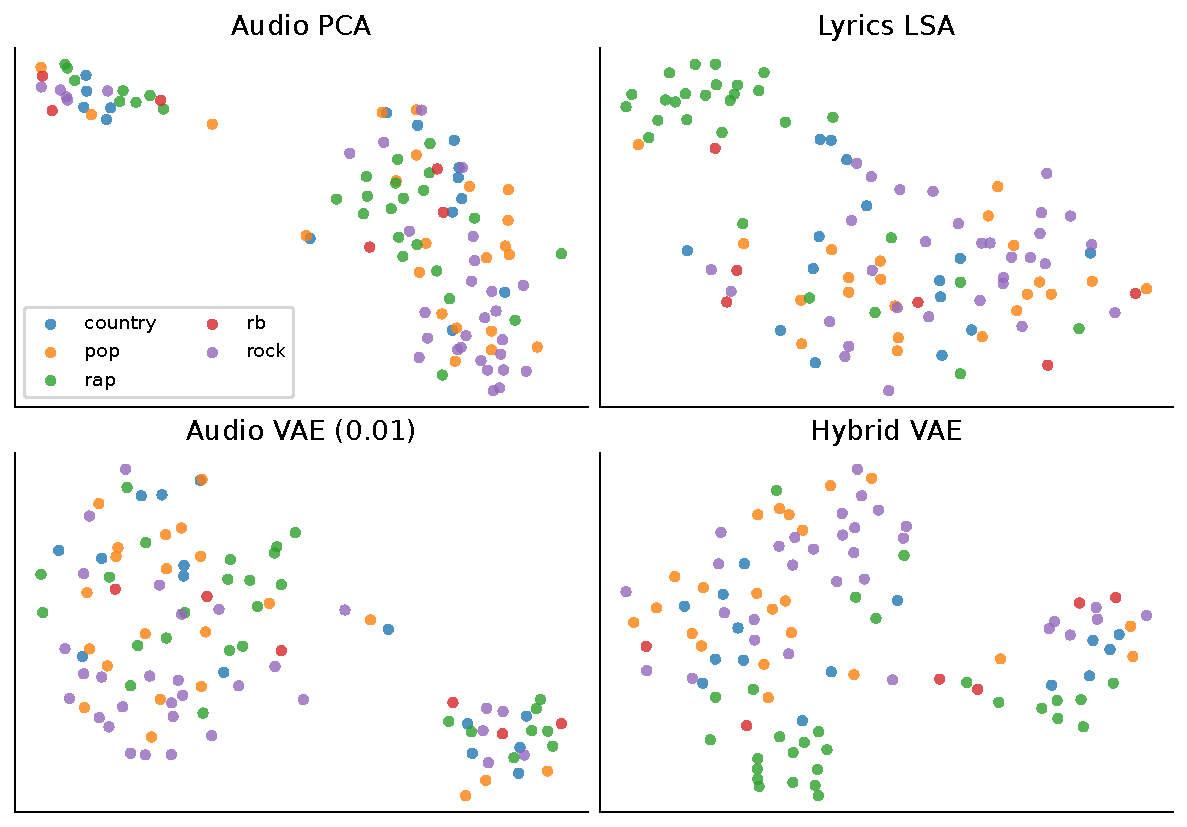
\includegraphics[width=\linewidth]{figures/rebuilt_tsne.pdf}
\caption{Test-set t-SNE, seed 11, perplexity 20, colored by genre for four
representations. Each panel is fitted separately; axes and distances across
panels are not comparable.}
\end{figure}
\begin{figure}[h]
\centering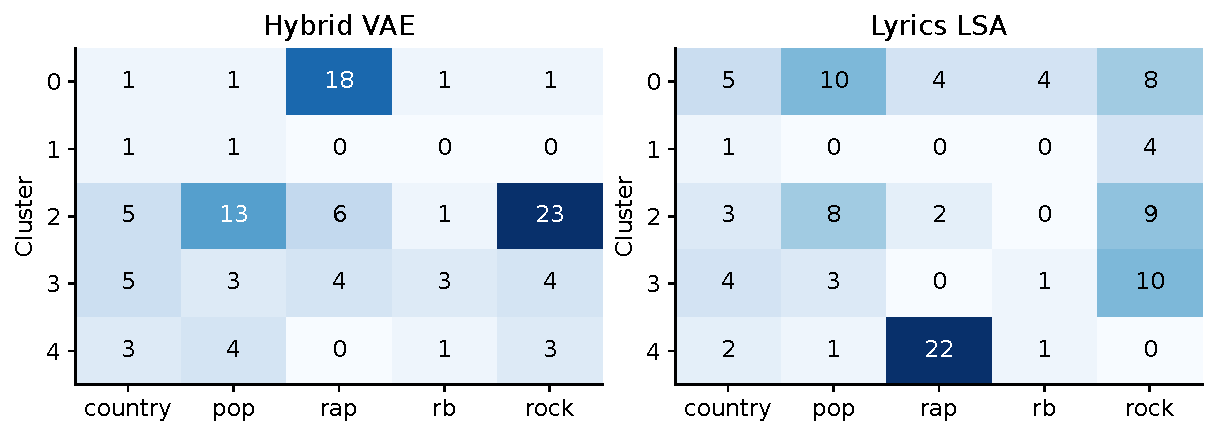
\includegraphics[width=\linewidth]{figures/rebuilt_genre_distribution.pdf}
\caption{Actual genre counts in the seed-11 held-out clusters. Cluster numbers
are arbitrary and cannot be matched across methods by their numeric ID.}
\end{figure}
\clearpage
\begin{figure}[h]
\centering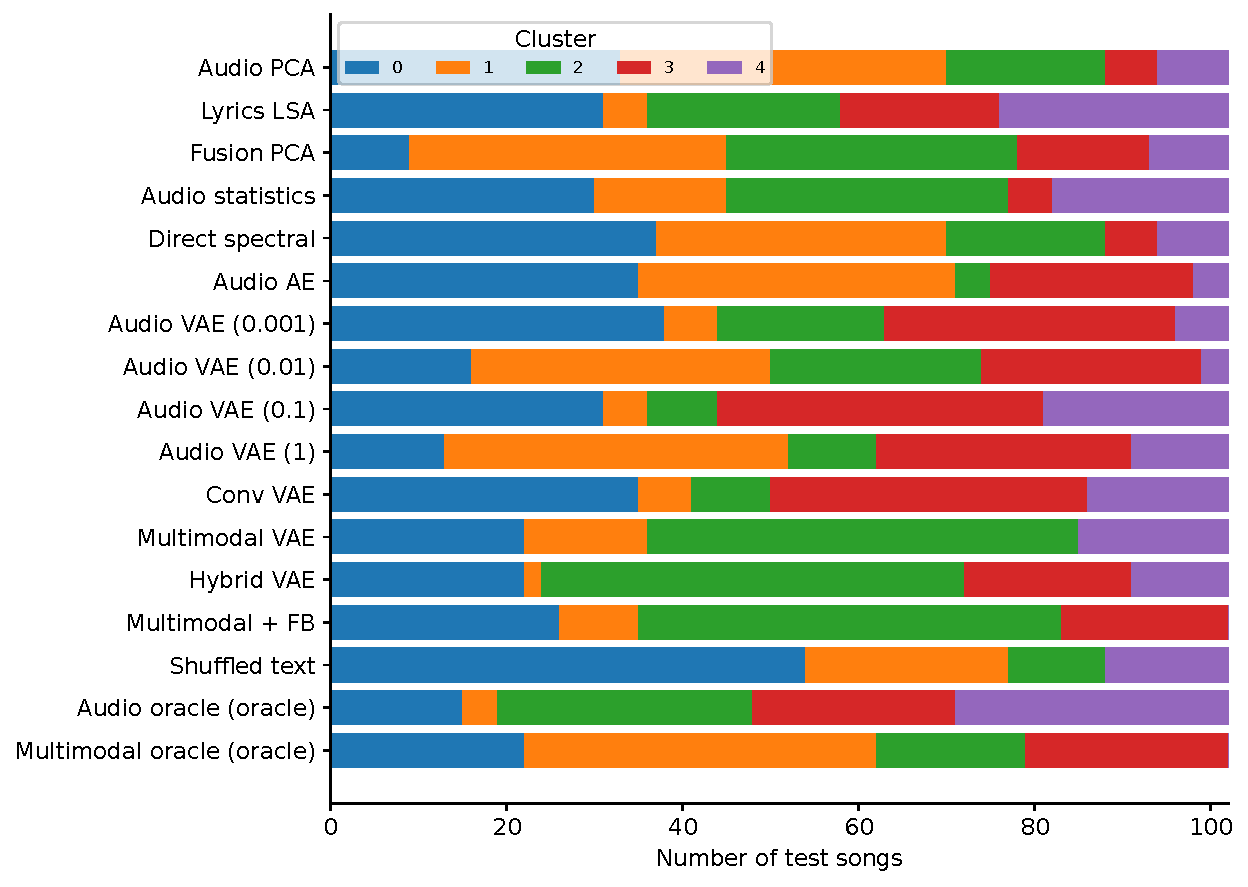
\includegraphics[width=\linewidth]{figures/rebuilt_cluster_sizes.pdf}
\caption{Test cluster sizes for seed 11, including separately identified genre
oracles and the shuffled-text control. Small or dominant clusters remain visible.}
\end{figure}
\begin{figure}[h]
\centering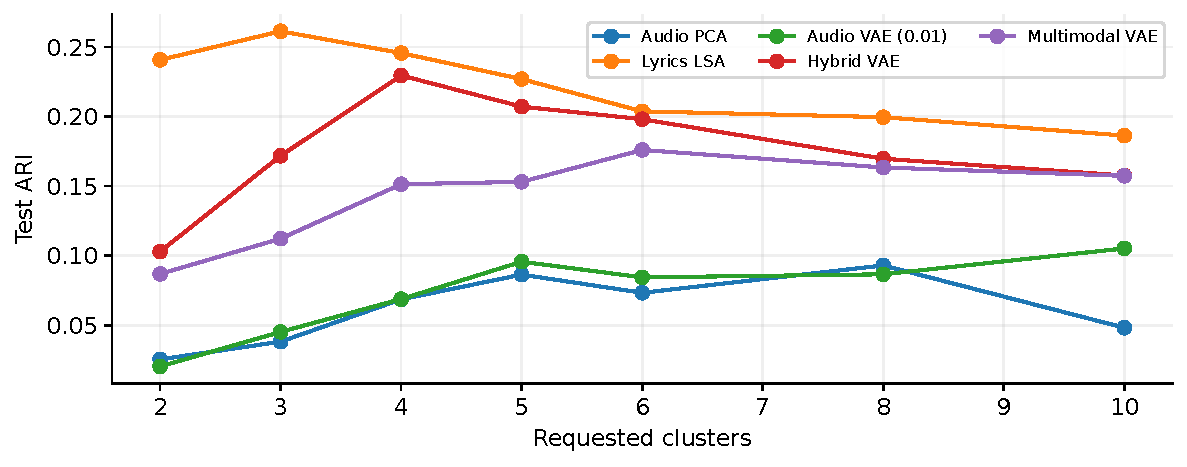
\includegraphics[width=\linewidth]{figures/rebuilt_k_sensitivity.pdf}
\caption{Sensitivity to the prespecified cluster-count grid. Lines show mean
test ARI across seeds. The grid is descriptive; no test-based $k$ is selected.}
\end{figure}
\clearpage
\begin{figure}[h]
\centering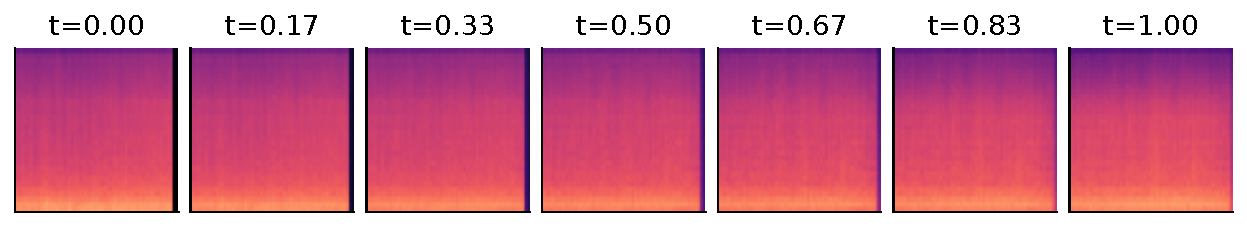
\includegraphics[width=\linewidth]{figures/rebuilt_interpolation.pdf}
\caption{Linear interpolation between two seed-11 audio-VAE posterior means
(first test country and rock examples). Smooth decoder output alone does not
establish musically meaningful interpolation.}
\end{figure}
\begin{figure}[h]
\centering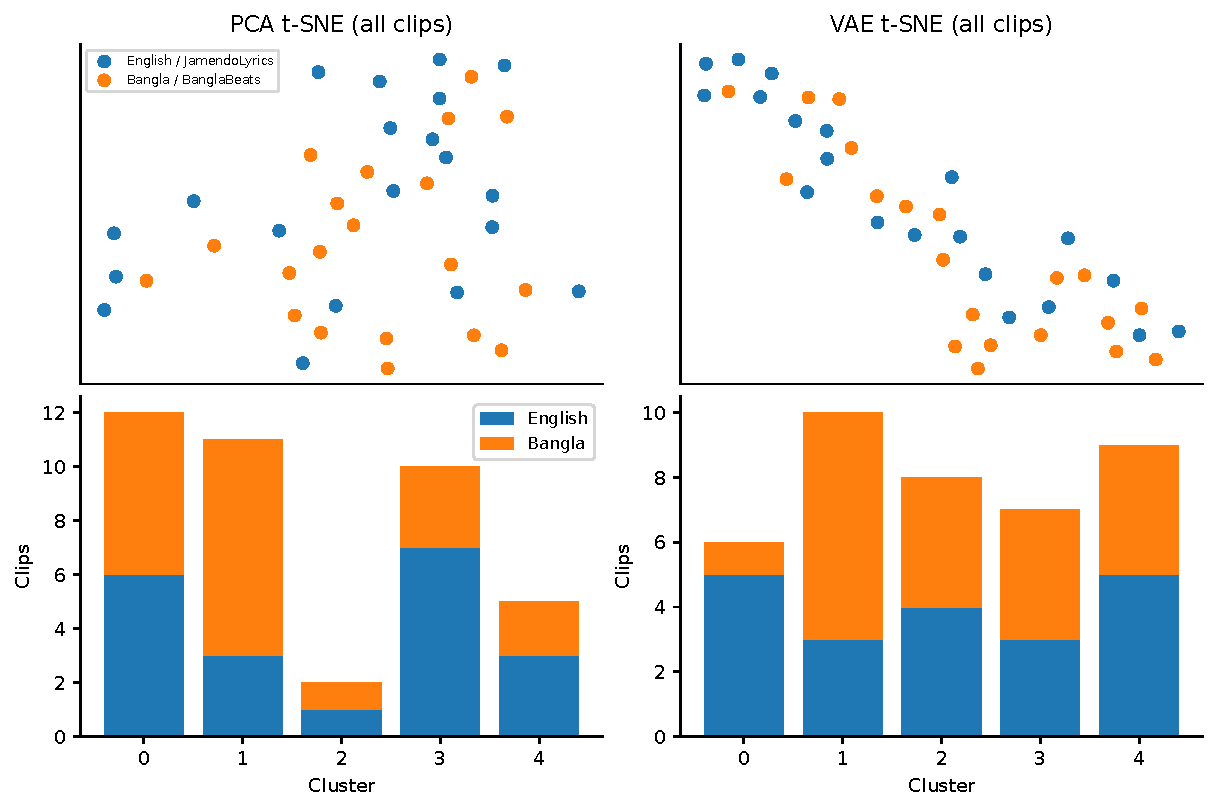
\includegraphics[width=\linewidth]{figures/bilingual.pdf}
\caption{Bilingual course demonstration: t-SNE colored by annotated language/source and actual language counts in the five seed-11 clusters. All 40 clips are included. Bengali original song IDs are unavailable, and language and source cannot be disentangled.}
\end{figure}

\clearpage
\section*{Research checklist (supplied 2024 template)}
This checklist documents the current research draft; it is not a declaration of submission to NeurIPS.
\begin{enumerate}

\item {\bf Claims}
    \item[] Question: Do the main claims made in the abstract and introduction accurately reflect the paper's contributions and scope?
    \item[] Answer: \answerYes{} 
    \item[] Justification: Sections 1 and 6 distinguish the verified empirical results, the bilingual feasibility study, and the limits on generalization.
    \item[] Guidelines:
    \begin{itemize}
        \item The answer NA means that the abstract and introduction do not include the claims made in the paper.
        \item The abstract and/or introduction should clearly state the claims made, including the contributions made in the paper and important assumptions and limitations. A No or NA answer to this question will not be perceived well by the reviewers. 
        \item The claims made should match theoretical and experimental results, and reflect how much the results can be expected to generalize to other settings. 
        \item It is fine to include aspirational goals as motivation as long as it is clear that these goals are not attained by the paper. 
    \end{itemize}

\item {\bf Limitations}
    \item[] Question: Does the paper discuss the limitations of the work performed by the authors?
    \item[] Answer: \answerYes{} 
    \item[] Justification: Section 7 describes data provenance, split size, source/language confounding, missing artist identifiers, and limits of the representation and evaluation.
    \item[] Guidelines:
    \begin{itemize}
        \item The answer NA means that the paper has no limitation while the answer No means that the paper has limitations, but those are not discussed in the paper. 
        \item The authors are encouraged to create a separate "Limitations" section in their paper.
        \item The paper should point out any strong assumptions and how robust the results are to violations of these assumptions (e.g., independence assumptions, noiseless settings, model well-specification, asymptotic approximations only holding locally). The authors should reflect on how these assumptions might be violated in practice and what the implications would be.
        \item The authors should reflect on the scope of the claims made, e.g., if the approach was only tested on a few datasets or with a few runs. In general, empirical results often depend on implicit assumptions, which should be articulated.
        \item The authors should reflect on the factors that influence the performance of the approach. For example, a facial recognition algorithm may perform poorly when image resolution is low or images are taken in low lighting. Or a speech-to-text system might not be used reliably to provide closed captions for online lectures because it fails to handle technical jargon.
        \item The authors should discuss the computational efficiency of the proposed algorithms and how they scale with dataset size.
        \item If applicable, the authors should discuss possible limitations of their approach to address problems of privacy and fairness.
        \item While the authors might fear that complete honesty about limitations might be used by reviewers as grounds for rejection, a worse outcome might be that reviewers discover limitations that aren't acknowledged in the paper. The authors should use their best judgment and recognize that individual actions in favor of transparency play an important role in developing norms that preserve the integrity of the community. Reviewers will be specifically instructed to not penalize honesty concerning limitations.
    \end{itemize}

\pagebreak
\item {\bf Theory Assumptions and Proofs}
    \item[] Question: For each theoretical result, does the paper provide the full set of assumptions and a complete (and correct) proof?
    \item[] Answer: \answerNA{} 
    \item[] Justification: No new theoretical result is claimed; the loss is specified as an implemented dimension-normalized objective.
    \item[] Guidelines:
    \begin{itemize}
        \item The answer NA means that the paper does not include theoretical results. 
        \item All the theorems, formulas, and proofs in the paper should be numbered and cross-referenced.
        \item All assumptions should be clearly stated or referenced in the statement of any theorems.
        \item The proofs can either appear in the main paper or the supplemental material, but if they appear in the supplemental material, the authors are encouraged to provide a short proof sketch to provide intuition. 
        \item Inversely, any informal proof provided in the core of the paper should be complemented by formal proofs provided in appendix or supplemental material.
        \item Theorems and Lemmas that the proof relies upon should be properly referenced. 
    \end{itemize}

    \item {\bf Experimental Result Reproducibility}
    \item[] Question: Does the paper fully disclose all the information needed to reproduce the main experimental results of the paper to the extent that it affects the main claims and/or conclusions of the paper (regardless of whether the code and data are provided or not)?
    \item[] Answer: \answerYes{} 
    \item[] Justification: Section 5 and Appendix A specify the runs and provide source/configuration/input hashes, saved splits and exact commands. Original raw extraction for the supplied corpus cannot be reconstructed, and no claim of raw-data reproducibility is made.
    \item[] Guidelines:
    \begin{itemize}
        \item The answer NA means that the paper does not include experiments.
        \item If the paper includes experiments, a No answer to this question will not be perceived well by the reviewers: Making the paper reproducible is important, regardless of whether the code and data are provided or not.
        \item If the contribution is a dataset and/or model, the authors should describe the steps taken to make their results reproducible or verifiable. 
        \item Depending on the contribution, reproducibility can be accomplished in various ways. For example, if the contribution is a novel architecture, describing the architecture fully might suffice, or if the contribution is a specific model and empirical evaluation, it may be necessary to either make it possible for others to replicate the model with the same dataset, or provide access to the model. In general. releasing code and data is often one good way to accomplish this, but reproducibility can also be provided via detailed instructions for how to replicate the results, access to a hosted model (e.g., in the case of a large language model), releasing of a model checkpoint, or other means that are appropriate to the research performed.
        \item While NeurIPS does not require releasing code, the conference does require all submissions to provide some reasonable avenue for reproducibility, which may depend on the nature of the contribution. For example
        \begin{enumerate}
            \item If the contribution is primarily a new algorithm, the paper should make it clear how to reproduce that algorithm.
            \item If the contribution is primarily a new model architecture, the paper should describe the architecture clearly and fully.
            \item If the contribution is a new model (e.g., a large language model), then there should either be a way to access this model for reproducing the results or a way to reproduce the model (e.g., with an open-source dataset or instructions for how to construct the dataset).
            \item We recognize that reproducibility may be tricky in some cases, in which case authors are welcome to describe the particular way they provide for reproducibility. In the case of closed-source models, it may be that access to the model is limited in some way (e.g., to registered users), but it should be possible for other researchers to have some path to reproducing or verifying the results.
        \end{enumerate}
    \end{itemize}


\item {\bf Open access to data and code}
    \item[] Question: Does the paper provide open access to the data and code, with sufficient instructions to faithfully reproduce the main experimental results, as described in supplemental material?
    \item[] Answer: \answerNo{} 
    \item[] Justification: Revised code and results are documented. The existing public repository contains byte-identical legacy inputs, but their original provenance and reuse rights remain unresolved. Public sources and access scripts are documented for the bilingual cohort.
    \item[] Guidelines:
    \begin{itemize}
        \item The answer NA means that paper does not include experiments requiring code.
        \item Please see the NeurIPS code and data submission guidelines (\url{https://nips.cc/public/guides/CodeSubmissionPolicy}) for more details.
        \item While we encourage the release of code and data, we understand that this might not be possible, so ``No'' is an acceptable answer. Papers cannot be rejected simply for not including code, unless this is central to the contribution (e.g., for a new open-source benchmark).
        \item The instructions should contain the exact command and environment needed to run to reproduce the results. See the NeurIPS code and data submission guidelines (\url{https://nips.cc/public/guides/CodeSubmissionPolicy}) for more details.
        \item The authors should provide instructions on data access and preparation, including how to access the raw data, preprocessed data, intermediate data, and generated data, etc.
        \item The authors should provide scripts to reproduce all experimental results for the new proposed method and baselines. If only a subset of experiments are reproducible, they should state which ones are omitted from the script and why.
        \item At submission time, to preserve anonymity, the authors should release anonymized versions (if applicable).
        \item Providing as much information as possible in supplemental material (appended to the paper) is recommended, but including URLs to data and code is permitted.
    \end{itemize}


\item {\bf Experimental Setting/Details}
    \item[] Question: Does the paper specify all the training and test details (e.g., data splits, hyperparameters, how they were chosen, type of optimizer, etc.) necessary to understand the results?
    \item[] Answer: \answerYes{} 
    \item[] Justification: Architectures, preprocessing, seeds, selection criterion, objective reductions and clustering parameters are specified in Sections 4--5 and configuration files.
    \item[] Guidelines:
    \begin{itemize}
        \item The answer NA means that the paper does not include experiments.
        \item The experimental setting should be presented in the core of the paper to a level of detail that is necessary to appreciate the results and make sense of them.
        \item The full details can be provided either with the code, in appendix, or as supplemental material.
    \end{itemize}

\item {\bf Experiment Statistical Significance}
    \item[] Question: Does the paper report error bars suitably and correctly defined or other appropriate information about the statistical significance of the experiments?
    \item[] Answer: \answerYes{} 
    \item[] Justification: Tables report sample standard deviations across five seeds. Appendix A gives exploratory paired group/seed bootstrap intervals and states their conditional scope; no confirmatory multiple-testing claim is made.
    \item[] Guidelines:
    \begin{itemize}
        \item The answer NA means that the paper does not include experiments.
        \item The authors should answer "Yes" if the results are accompanied by error bars, confidence intervals, or statistical significance tests, at least for the experiments that support the main claims of the paper.
        \item The factors of variability that the error bars are capturing should be clearly stated (for example, train/test split, initialization, random drawing of some parameter, or overall run with given experimental conditions).
        \item The method for calculating the error bars should be explained (closed form formula, call to a library function, bootstrap, etc.)
        \item The assumptions made should be given (e.g., Normally distributed errors).
        \item It should be clear whether the error bar is the standard deviation or the standard error of the mean.
        \item It is OK to report 1-sigma error bars, but one should state it. The authors should preferably report a 2-sigma error bar than state that they have a 96\% CI, if the hypothesis of Normality of errors is not verified.
        \item For asymmetric distributions, the authors should be careful not to show in tables or figures symmetric error bars that would yield results that are out of range (e.g. negative error rates).
        \item If error bars are reported in tables or plots, The authors should explain in the text how they were calculated and reference the corresponding figures or tables in the text.
    \end{itemize}

\item {\bf Experiments Compute Resources}
    \item[] Question: For each experiment, does the paper provide sufficient information on the computer resources (type of compute workers, memory, time of execution) needed to reproduce the experiments?
    \item[] Answer: \answerYes{} 
    \item[] Justification: Experiments used an Apple M1 MacBook Air with 8 GB physical memory and four CPU threads. Section 5 reports measured training wall time; manifests record package versions. Peak memory was not measured.
    \item[] Guidelines:
    \begin{itemize}
        \item The answer NA means that the paper does not include experiments.
        \item The paper should indicate the type of compute workers CPU or GPU, internal cluster, or cloud provider, including relevant memory and storage.
        \item The paper should provide the amount of compute required for each of the individual experimental runs as well as estimate the total compute. 
        \item The paper should disclose whether the full research project required more compute than the experiments reported in the paper (e.g., preliminary or failed experiments that didn't make it into the paper). 
    \end{itemize}
    
\item {\bf Code Of Ethics}
    \item[] Question: Does the research conducted in the paper conform, in every respect, with the NeurIPS Code of Ethics \url{https://neurips.cc/public/EthicsGuidelines}?
    \item[] Answer: \answerNo{} 
    \item[] Justification: The supplied corpus has unresolved provenance and license metadata. This is disclosed rather than asserting that public-release requirements are verified.
    \item[] Guidelines:
    \begin{itemize}
        \item The answer NA means that the authors have not reviewed the NeurIPS Code of Ethics.
        \item If the authors answer No, they should explain the special circumstances that require a deviation from the Code of Ethics.
        \item The authors should make sure to preserve anonymity (e.g., if there is a special consideration due to laws or regulations in their jurisdiction).
    \end{itemize}


\pagebreak
\item {\bf Broader Impacts}
    \item[] Question: Does the paper discuss both potential positive societal impacts and negative societal impacts of the work performed?
    \item[] Answer: \answerYes{} 
    \item[] Justification: Section 7 discusses cultural coverage, inappropriate semantic interpretations, training-material retention and redistribution constraints.
    \item[] Guidelines:
    \begin{itemize}
        \item The answer NA means that there is no societal impact of the work performed.
        \item If the authors answer NA or No, they should explain why their work has no societal impact or why the paper does not address societal impact.
        \item Examples of negative societal impacts include potential malicious or unintended uses (e.g., disinformation, generating fake profiles, surveillance), fairness considerations (e.g., deployment of technologies that could make decisions that unfairly impact specific groups), privacy considerations, and security considerations.
        \item The conference expects that many papers will be foundational research and not tied to particular applications, let alone deployments. However, if there is a direct path to any negative applications, the authors should point it out. For example, it is legitimate to point out that an improvement in the quality of generative models could be used to generate deepfakes for disinformation. On the other hand, it is not needed to point out that a generic algorithm for optimizing neural networks could enable people to train models that generate Deepfakes faster.
        \item The authors should consider possible harms that could arise when the technology is being used as intended and functioning correctly, harms that could arise when the technology is being used as intended but gives incorrect results, and harms following from (intentional or unintentional) misuse of the technology.
        \item If there are negative societal impacts, the authors could also discuss possible mitigation strategies (e.g., gated release of models, providing defenses in addition to attacks, mechanisms for monitoring misuse, mechanisms to monitor how a system learns from feedback over time, improving the efficiency and accessibility of ML).
    \end{itemize}
    
\item {\bf Safeguards}
    \item[] Question: Does the paper describe safeguards that have been put in place for responsible release of data or models that have a high risk for misuse (e.g., pretrained language models, image generators, or scraped datasets)?
    \item[] Answer: \answerNA{} 
    \item[] Justification: No high-risk model or publicly redistributed scraped corpus is released by this work. Local access and licensing limitations are documented.
    \item[] Guidelines:
    \begin{itemize}
        \item The answer NA means that the paper poses no such risks.
        \item Released models that have a high risk for misuse or dual-use should be released with necessary safeguards to allow for controlled use of the model, for example by requiring that users adhere to usage guidelines or restrictions to access the model or implementing safety filters. 
        \item Datasets that have been scraped from the Internet could pose safety risks. The authors should describe how they avoided releasing unsafe images.
        \item We recognize that providing effective safeguards is challenging, and many papers do not require this, but we encourage authors to take this into account and make a best faith effort.
    \end{itemize}

\item {\bf Licenses for existing assets}
    \item[] Question: Are the creators or original owners of assets (e.g., code, data, models), used in the paper, properly credited and are the license and terms of use explicitly mentioned and properly respected?
    \item[] Answer: \answerNo{} 
    \item[] Justification: External datasets and source revisions are credited. The supplied corpus and the BanglaBeats release lack sufficient verified licensing information; this remains a release blocker.
    \item[] Guidelines:
    \begin{itemize}
        \item The answer NA means that the paper does not use existing assets.
        \item The authors should cite the original paper that produced the code package or dataset.
        \item The authors should state which version of the asset is used and, if possible, include a URL.
        \item The name of the license (e.g., CC-BY 4.0) should be included for each asset.
        \item For scraped data from a particular source (e.g., website), the copyright and terms of service of that source should be provided.
        \item If assets are released, the license, copyright information, and terms of use in the package should be provided. For popular datasets, \url{paperswithcode.com/datasets} has curated licenses for some datasets. Their licensing guide can help determine the license of a dataset.
        \item For existing datasets that are re-packaged, both the original license and the license of the derived asset (if it has changed) should be provided.
        \item If this information is not available online, the authors are encouraged to reach out to the asset's creators.
    \end{itemize}

\item {\bf New Assets}
    \item[] Question: Are new assets introduced in the paper well documented and is the documentation provided alongside the assets?
    \item[] Answer: \answerYes{} 
    \item[] Justification: New code, configurations, checkpoints and results are documented in the local package and README. This does not imply a public licensed data release.
    \item[] Guidelines:
    \begin{itemize}
        \item The answer NA means that the paper does not release new assets.
        \item Researchers should communicate the details of the dataset/code/model as part of their submissions via structured templates. This includes details about training, license, limitations, etc. 
        \item The paper should discuss whether and how consent was obtained from people whose asset is used.
        \item At submission time, remember to anonymize your assets (if applicable). You can either create an anonymized URL or include an anonymized zip file.
    \end{itemize}

\item {\bf Crowdsourcing and Research with Human Subjects}
    \item[] Question: For crowdsourcing experiments and research with human subjects, does the paper include the full text of instructions given to participants and screenshots, if applicable, as well as details about compensation (if any)? 
    \item[] Answer: \answerNA{} 
    \item[] Justification: No crowdsourcing or human-subject experiment was performed.
    \item[] Guidelines:
    \begin{itemize}
        \item The answer NA means that the paper does not involve crowdsourcing nor research with human subjects.
        \item Including this information in the supplemental material is fine, but if the main contribution of the paper involves human subjects, then as much detail as possible should be included in the main paper. 
        \item According to the NeurIPS Code of Ethics, workers involved in data collection, curation, or other labor should be paid at least the minimum wage in the country of the data collector. 
    \end{itemize}

\pagebreak
\item {\bf Institutional Review Board (IRB) Approvals or Equivalent for Research with Human Subjects}
    \item[] Question: Does the paper describe potential risks incurred by study participants, whether such risks were disclosed to the subjects, and whether Institutional Review Board (IRB) approvals (or an equivalent approval/review based on the requirements of your country or institution) were obtained?
    \item[] Answer: \answerNA{} 
    \item[] Justification: No new human-subject experiment was performed; dataset reuse limitations are stated.
    \item[] Guidelines:
    \begin{itemize}
        \item The answer NA means that the paper does not involve crowdsourcing nor research with human subjects.
        \item Depending on the country in which research is conducted, IRB approval (or equivalent) may be required for any human subjects research. If you obtained IRB approval, you should clearly state this in the paper. 
        \item We recognize that the procedures for this may vary significantly between institutions and locations, and we expect authors to adhere to the NeurIPS Code of Ethics and the guidelines for their institution. 
        \item For initial submissions, do not include any information that would break anonymity (if applicable), such as the institution conducting the review.
    \end{itemize}

\end{enumerate}

\end{document}
